\subsection{Examples}
\label{sec:examples}
Another experiment we ran was to evaluate the accuracy of the classifier in a
setting where, if the correct token is not within the top few predictions, the
user types in one or more characters to ``home in'' on the correct prediction.
Figure~\ref{fig:codeexample} shows the results for this experiment. In this
experiment, a character is colored in green if the token is correctly predicted
(i.e., top prediction) before that character is typed. It is colored in yellow
if the token is among the top 5 before typing that character, and colored in red
if the token is not among the top 5. So, for example, in the first line in the
token
{\tt struct}, the character {\tt s} is in yellow since before typing {\tt s}, the
token {\tt struct} was among the top 5. After typing {\tt s}, the top prediction
was {\tt struct}, and thus the characters {\tt truct} are all in green. We
can see that, for example, entire sequences of code such as {\tt \{
PCI\_VDEVICE(SUNDANCE, } are predicted correctly without typing anything.
\begin{figure}[h]
  \centering
  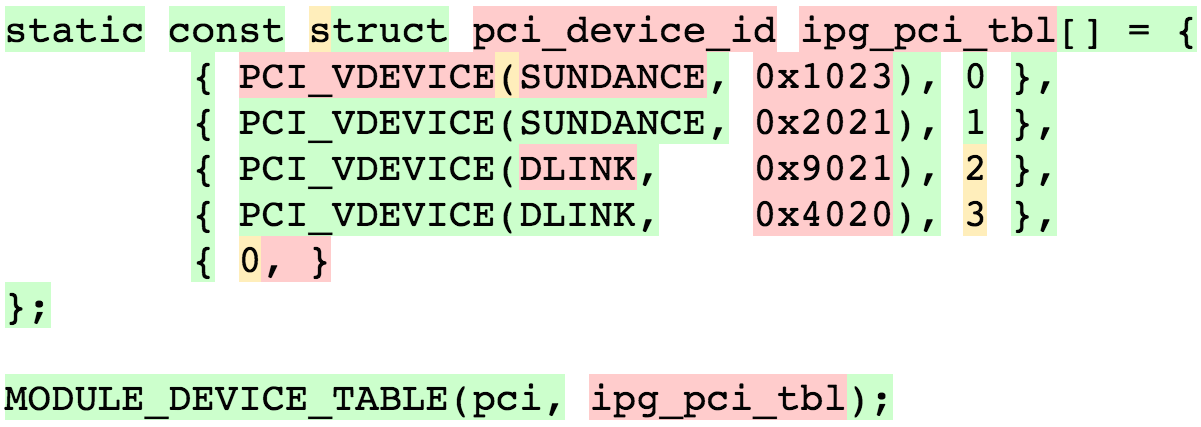
\includegraphics[width=\linewidth]{figs/example3.png}
  \caption{Code example with per-character predictions}
  \label{fig:codeexample}
\end{figure}

\subsubsection{Importance of Positional Tokens}
From Figure~\ref{fig:codeexample} we can also see the importance of positional
tokens. The tokens {\tt PCI\_VDEVICE} and {\tt SUNDANCE} are both not keywords
(i.e., not frequently observed in the codebase), and yet were predicted
correctly by our method the second time they were used (in line 3). If we chose
to ignore such tokens instead, we would not have been able to predict such
tokens correctly in a majority of cases.

\subsubsection{Learning Frequently Occurring Patterns}
We also found several interesting patterns that are predicted correctly by our
system. An example of such a pattern is given in
Figures~\ref{fig:conditional1}~\&~\ref{fig:conditional2}. In these figures, each
character is color coded as before, and some additional information is also
shown. The top 5 predictions at the position of interest (shown in red border),
are shown in a blue box. Also, the value of attention for each token in the
prediction window are shown color coded in sky-blue, where deeper blue is
indicative of more attention (for reference, the first {\tt if} tokens in both
of these two cases have an attention value of $\approx$ 1).

\begin{figure}
  \centering
\begin{subfigure}{\linewidth}
  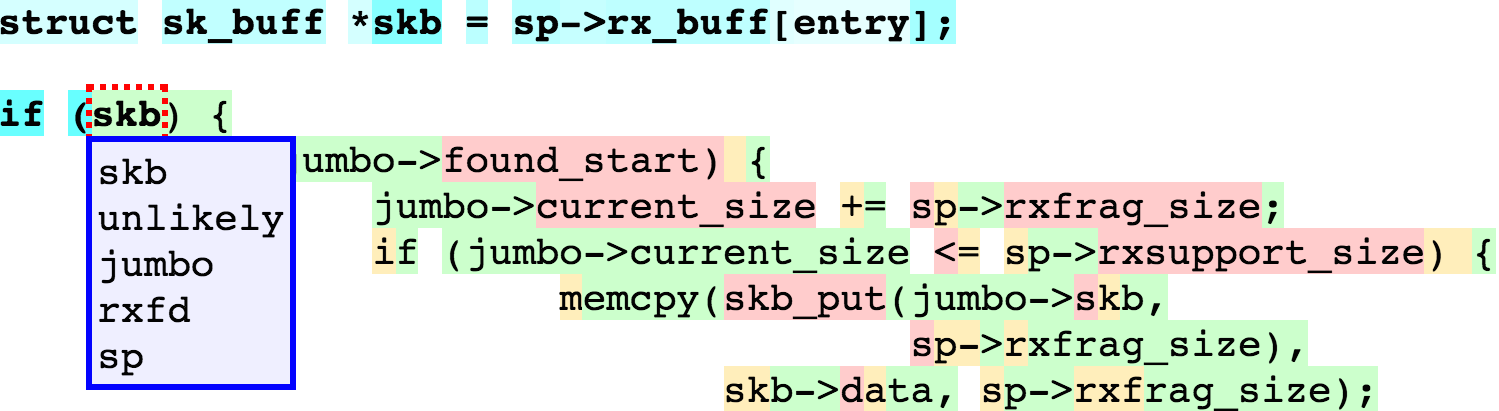
\includegraphics[width=\linewidth]{figs/example8.png}
  \caption{Example 1}
  \label{fig:conditional1}
\end{subfigure}
\begin{subfigure}{\linewidth}
  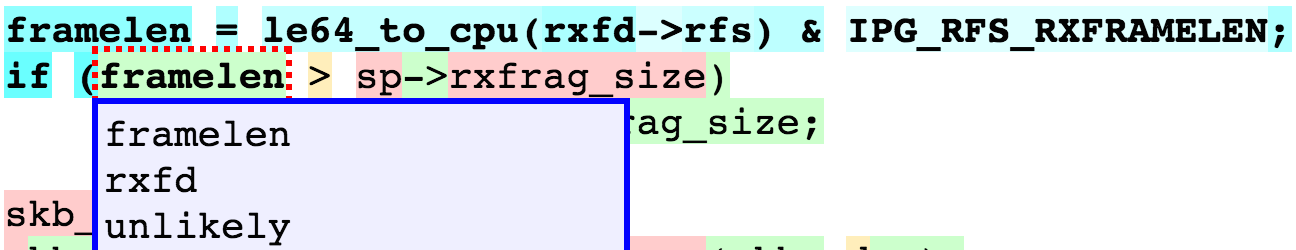
\includegraphics[width=\linewidth]{figs/example9.png}
  \caption{Example 2}
  \label{fig:conditional2}
\end{subfigure}
  \caption{Definition before {\tt if} pattern}
  \label{fig:ifpattern}
\end{figure}

Here, a variable is assigned to right before an {\tt if} statement, and the
prediction is that the variable will be immediately used inside the {\tt if}
condition. This is a common pattern in Linux code, where if the condition inside
{\tt if} is too long, it is broken up into an assignment and a subsequent
conditional.

Also, in the figure the top 5 predictions for each case is given in the blue
box. We can see that {\tt unlikely} is a common prediction, since {\tt if
(unlikely(condition))} is a common pattern in Linux code to check for unlikely
edge cases such as error conditions.

We can also see that the attention of the models is relatively high at the
correct predictions ({\tt skb} and {\tt framelen} in the first and second cases
respectively). This shows that even a single layer model can be expected to
fairly reliably predict the next token (since the attention is derived from a
single non-linear layer).

A few more interesting examples are shown in Figure~\ref{fig:moreexamples}.

